\chapter{Experiments and Evaluation}
\label{experiments}

This section aims at evaluating the proposed metric in Chapter \ref{design} against state of the art metrics for trees comparison mentioned in Chapter \ref{related}. We test these metrics in various scenarios and datasets: synthetic datasets give us a possibility to better understand the behaviour of metrics on simple examples and quantitatively measure the quality. In contrast, real datasets help to understand the scaling and generalisation potential of the metric regarding the requirements introduced in Chapter \ref{related}. All results are scaled to lay in the interval [0,1].

%The code is available at \url{https://github.com/}. Complete information on the experiments (e.g. configurations, evaluation results, etc.) is available in appendix \ref{appendix}.
%
%# TODO

\section{Experimental Setup}
\paragraph{Hardware stack.}The experiments are run on a computer equipped with an Intel Core i7 8-Core Processor and 16 GB of RAM, with a Ubuntu 20.04 OS.

\paragraph{Software stack.}For the practical implementations of the algorithms, metrics, and experiments, the Python language was chosen. We also rely on open source libraries and datasets. For example, the ETE Toolkit \cite{ete3} was used to encapsulate a tree structure. Other beneficial libraries which contain many metrics and visualisations implemented for clustering are scikit-learn \cite{scikit-learn} and scipy \cite{2020SciPy}. We used state of the art hierarchical clustering algorithms for graphs which are efficiently implemented in scikit-network package \cite{scikit-network}.    
\section{Syntactic data}

\paragraph{Simple structure}

\begin{figure}[h]
	\centering
	\subfigure{
		\centering
		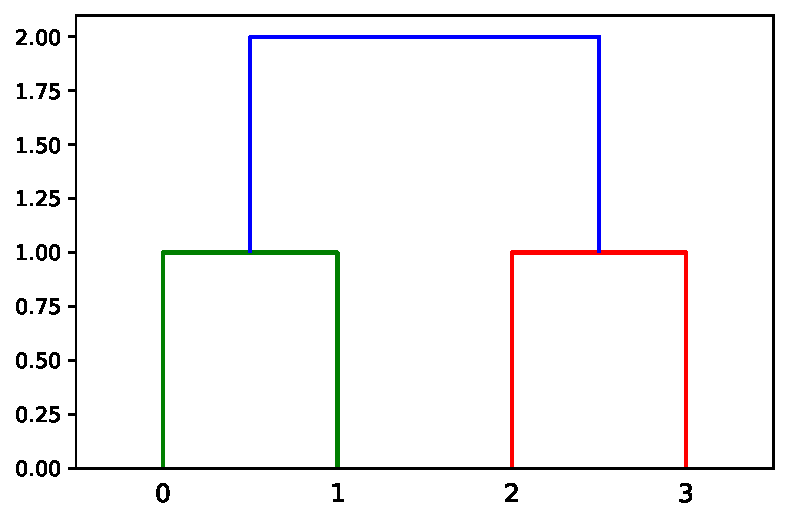
\includegraphics[width=0.46\textwidth,keepaspectratio=true]{figures/1-simple-dendrogram_0.pdf}
		\label{fig:simple_dendeogram_a}
	}
	\subfigure{
		\centering
		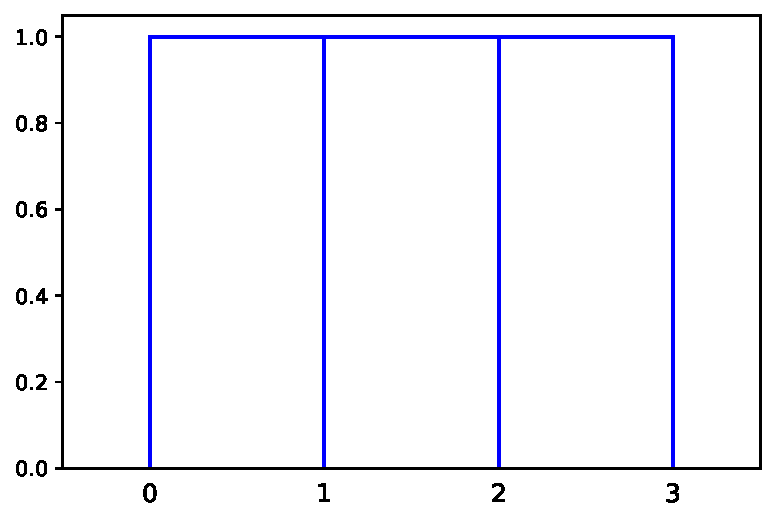
\includegraphics[width=0.46\textwidth,keepaspectratio=true]{figures/1-simple-dendrogram_1.pdf}
		\label{fig:simple_dendeogram_b}
	}
	\subfigure{
		\centering
		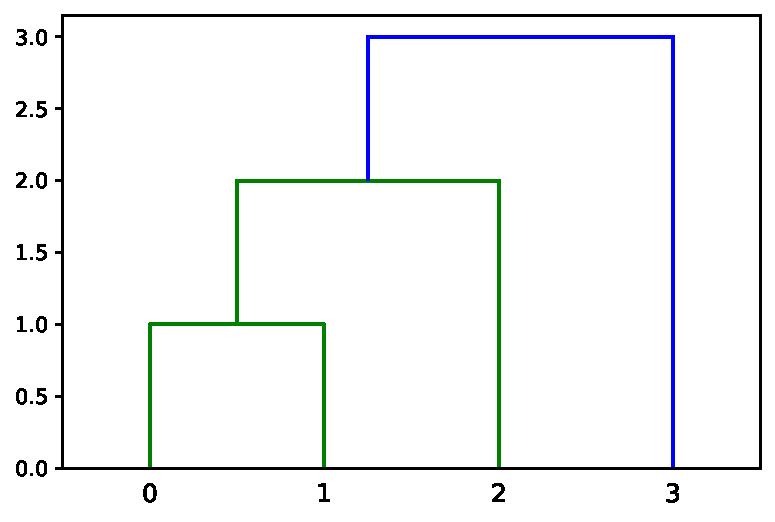
\includegraphics[width=0.46\textwidth,keepaspectratio=true]{figures/1-simple-dendrogram_2.pdf}
		\label{fig:simple_dendeogram_c}
	}
	\subfigure{
		\centering
		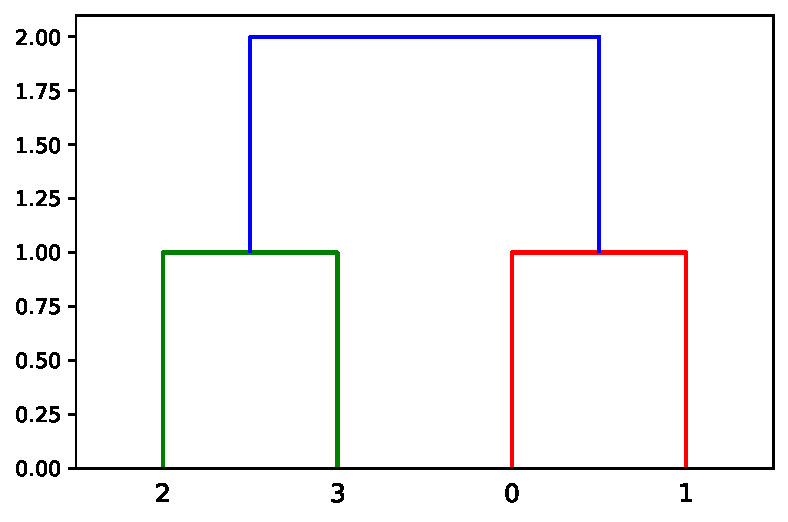
\includegraphics[width=0.46\textwidth,keepaspectratio=true]{figures/1-simple-dendrogram_3.pdf}
		\label{fig:simple_dendeogram_d}
	}
	\caption{Simple Experiment - example dendrograms with different structure.}
	\label{fig:simple_dendeogram}
\end{figure}

In this experiment, we generated base elements from more complex dendrograms and trees. The goal is to understand the behaviour of selected metrics on simple structures like the ones displayed in Figure \ref{fig:simple_dendeogram} and apply them for analysis of more complex scenarios. In Figure \ref{fig:simple_dendeogram_a} and \ref{fig:simple_dendeogram_d} we can see a binary tree with 4 leaves, the only difference between these 2 trees is that we switched right and left subtrees. Figure \ref{fig:simple_dendeogram_b} represents a trivial tree that does not contain any information since each node either represents a separated cluster with one element or they all belong to one cluster with 4 elements. Finally, in Figure \ref{fig:simple_dendeogram_c} we see a caterpillar tree that on every level adds one node to an already existing cluster. 


\begin{table}[H]
	\centering
	\caption{Simple experiment - similarity matrix.  \label{simple_dendeogram_similarity}}
	\subfigure[TAMI.]{
		\centering
		\begin{tabular}{lllll}
\toprule
{} &     a &  b &     c &     d \\
\midrule
a &  0.46 & -1 &  0.29 &  0.46 \\
b &    -1 & -1 &    -1 &    -1 \\
c &  0.29 & -1 &  0.36 &  0.29 \\
d &  0.46 & -1 &  0.29 &  0.46 \\
\bottomrule
\end{tabular}

		\label{simple_dendeogram_similarity_ami}
	}
	\subfigure[TPAMI.]{
		\begin{tabular}{lllll}
\toprule
{} &     a &  b &     c &     d \\
\midrule
a &  0.17 & -1 &  0.09 &  0.17 \\
b &    -1 & -1 &    -1 &    -1 \\
c &  0.09 & -1 &  0.09 &  0.09 \\
d &  0.17 & -1 &  0.09 &  0.17 \\
\bottomrule
\end{tabular}

		\label{simple_dendeogram_similarity_pami}
	}
	\subfigure[RF.]{
		\begin{tabular}{lllll}
\toprule
{} &  a &  b &  c &  d \\
\midrule
a &  1 &  0 &  1 &  1 \\
b &  0 &  0 &  0 &  0 \\
c &  1 &  0 &  1 &  1 \\
d &  1 &  0 &  1 &  1 \\
\bottomrule
\end{tabular}

		\label{simple_dendeogram_similarity_rf}
	}
	\subfigure[ZSS.]{
		\begin{tabular}{lllll}
\toprule
{} &     a &     b &     c &     d \\
\midrule
a &     1 &  0.83 &  0.79 &  0.71 \\
b &  0.83 &     1 &  0.83 &   0.5 \\
c &  0.79 &  0.83 &     1 &   0.5 \\
d &  0.71 &   0.5 &   0.5 &     1 \\
\bottomrule
\end{tabular}

		\label{simple_dendeogram_similarity_zss}
	}
\end{table}


The experiment's results of comparing similarity in all-to-all settings can be seen in Table \ref{simple_dendeogram_similarity}. As shown, TAMI and TPAMI metrics have very similar results, different only by a scale factor. Flat clustering Figure \ref{fig:simple_dendeogram_b} receives 0 scores in all steps because it does not have any information in its structure. TAMI and TPAMI results in the same score to \ref{fig:simple_dendeogram_a} and \ref{fig:simple_dendeogram_d} as it was expected since they hold the same structure. The only noticeable contrast is the similarity between the caterpillar tree and binary tree: TAMI gives a lower score to the binary tree than to the caterpillar and identifies 3 clusters in both trees as an optimal number of clusters, shown in Table \ref{fig:simple_dendeogram_n_clusters}. According to TPAMI's results in Table \ref{simple_dendeogram_similarity_pami}, it tends to stop early and going less deep into the tree's structure. 

RF results in Table \ref{simple_dendeogram_similarity_rf} look very binary: we only see values 1 and 0. RF metric is not able to precisely capture differences in structures of the given trees. 

The last metric used for consideration was TED: it shows better results than RF by identifying trees' structural differences. However, a noticeable drawback its disability to adjust for different cluster's orders. Besides, dendrograms \ref{fig:simple_dendeogram_a} and \ref{fig:simple_dendeogram_d} have distinct similarities. Also, this metric finds similarities between trivial clustering and other trees, which is not desired. 

\begin{table}[H]
	\caption{Simple experiment - optimal number of clusters. \label{fig:simple_dendeogram_n_clusters}}
	\centering
	\subfigure[TAMI.]{
		\centering
		\begin{tabular}{lllll}
\toprule
{} &       a &       b &       c &       d \\
\midrule
a &  (2, 2) &  (0, 0) &  (3, 3) &  (2, 2) \\
b &  (0, 0) &  (0, 0) &  (0, 0) &  (0, 0) \\
c &  (3, 3) &  (0, 0) &  (2, 2) &  (3, 3) \\
d &  (2, 2) &  (0, 0) &  (3, 3) &  (2, 2) \\
\bottomrule
\end{tabular}
 
	}
	\subfigure[TPAMI.]{
		\begin{tabular}{lllll}
\toprule
{} &       a &       b &       c &       d \\
\midrule
a &  (2, 2) &  (0, 0) &  (2, 3) &  (2, 2) \\
b &  (0, 0) &  (0, 0) &  (0, 0) &  (0, 0) \\
c &  (3, 2) &  (0, 0) &  (2, 2) &  (3, 2) \\
d &  (2, 2) &  (0, 0) &  (2, 3) &  (2, 2) \\
\bottomrule
\end{tabular}

	}
\end{table}

The following two instances are intended to demonstrate the properties of TAMI and TPAMI metrics.

\begin{figure}[H]
	\centering
	\subfigure{
		\centering
		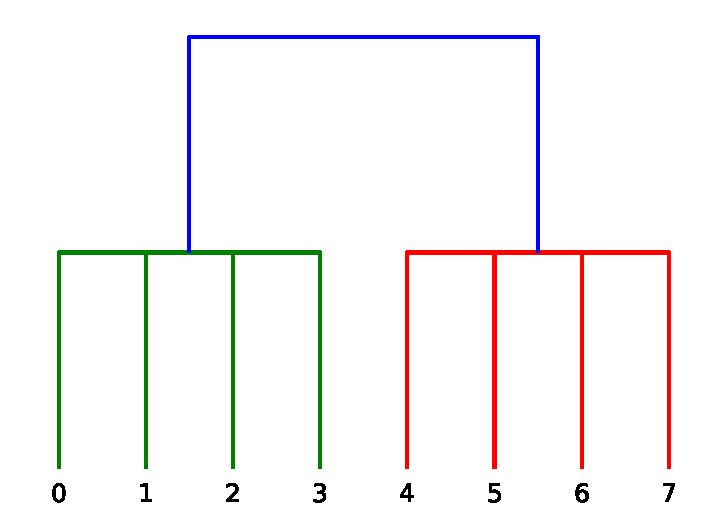
\includegraphics[width=0.46\textwidth,keepaspectratio=true]{figures/1-simple_results_tree_8_leaves_2_clusters.pdf}
		\label{fig:simple_dendeogram_aa}
	}
	\subfigure{
		\centering
		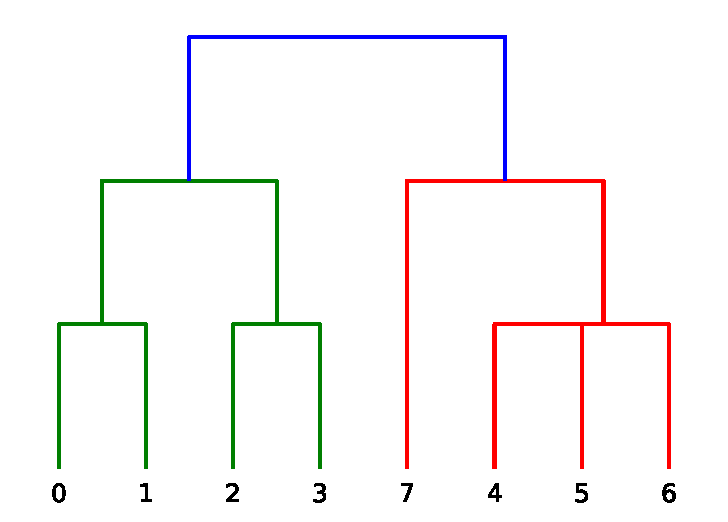
\includegraphics[width=0.46\textwidth,keepaspectratio=true]{figures/1-simple_results_tree_8_leaves_6_clusters.pdf}
		\label{fig:simple_dendeogram_bb}
	}
	\caption{Simple Experiment - tree \ref{fig:simple_dendeogram_aa} is a subtree of \ref{fig:simple_dendeogram_bb}.}
	\label{fig:simple_trees_comparison_2}
\end{figure}

First, let's consider that one tree is a subtree (sub clustering) of the second tree, in Figure \ref{fig:simple_trees_comparison_2} we see that if we collapse all subtrees in \ref{fig:simple_dendeogram_bb} then it will have the same structure as \ref{fig:simple_dendeogram_aa}, so we can say that one tree is a subcase of another. According to Information Theory, level 2 in tree \ref{fig:simple_dendeogram_aa} contains all information. Going deeper in any subtrees will not contribute any additional information, which results in the optimal number of clusters equal to 2 for both trees. We observe this behaviour by using TAMI and TPAMI on these trees: both metrics show the clusters' optimal number of 2 and similarity 0.62 and 0.14, respectively. Although both scores are not normalised and give only a relative understanding of similarity, our metrics can correctly identify the optimal number of clusters. 

\begin{figure}[H]
	\centering
	\subfigure{
		\centering
		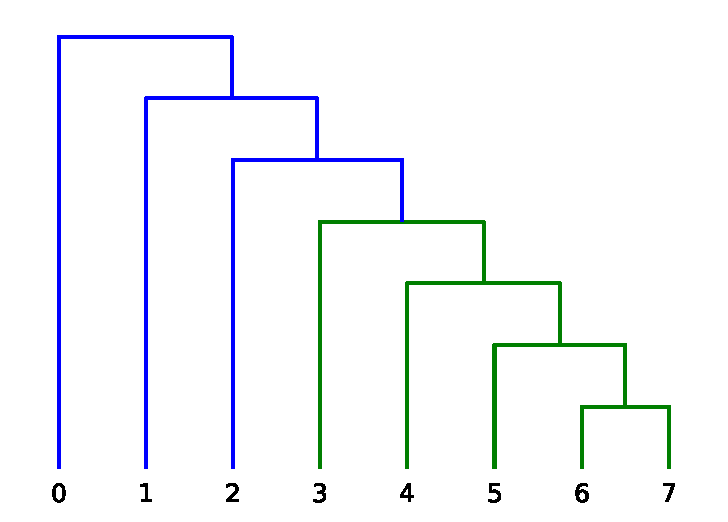
\includegraphics[width=0.46\textwidth,keepaspectratio=true]{figures/1-syntatic-tree-caterpillar-example.pdf}
		\label{fig:simple_tree_a}
	}
	\subfigure{
		\centering
		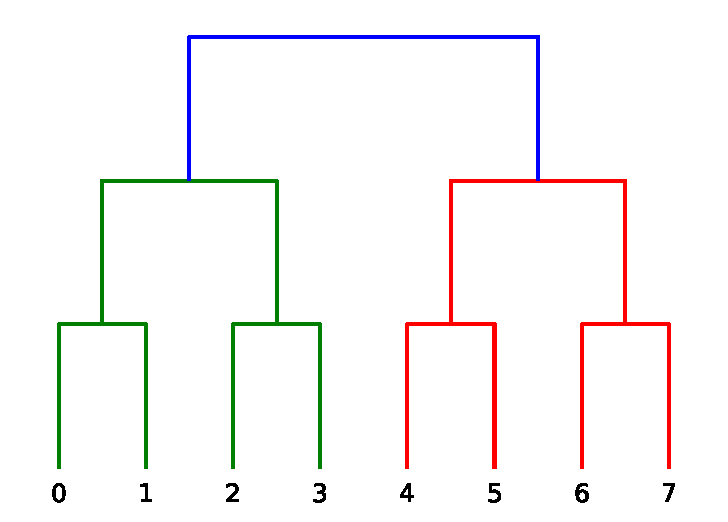
\includegraphics[width=0.46\textwidth,keepaspectratio=true]{figures/1-syntatic-tree-binary-example.pdf}
		\label{fig:simple_tree_b}
	}
	\caption{Simple Experiment - caterpillar and fully binary trees with 8 leaves.}
	\label{fig:simple_trees_comparison}
\end{figure}

Finally, we compare a caterpillar tree with a fully binary tree with 8 leaves. Intuitively, the best clustering is achieved by expanding all nodes in the left subtree of tree \ref{fig:simple_tree_b} and keeping the right(left) subtree as one complete cluster. It results in 5 clusters: 4 clusters with 1 element and one cluster of 4. Simultaneously, in the caterpillar tree \ref{fig:simple_tree_a} by sequentially going down till the 5th level, we obtain an identical distribution of nodes. After executing TAMI and TPAMI metrics, we obtain 5 clusters as the optimal number for both trees. 

\paragraph{Clustering}
Now let's consider a bit more complex example. This experiment is intended to demonstrate the behaviour of the Mutual Information, Adjusted Mutual Information, Pairwise Adjusted Mutual Information, Expected Mutual Information and Entropy in clustering scenario to measure the similarity between ground truth partitioning and predicted one, depending on the parameter $k$ in K-means clustering algorithm. 
For this experiment, we generate $M=10$ isotropic Gaussian blobs of equal size $n=50$, which overall results in $N=500$ data samples. Then we apply the K-Means algorithm with parameter $k$ ranging from 2 to 100 with step 8. We measure similarity between predicted and ground-truth clusterings. For generalisation purposes, we repeat the experiment 10 times and average the results. 

\begin{figure}[H]
	\begin{center}
		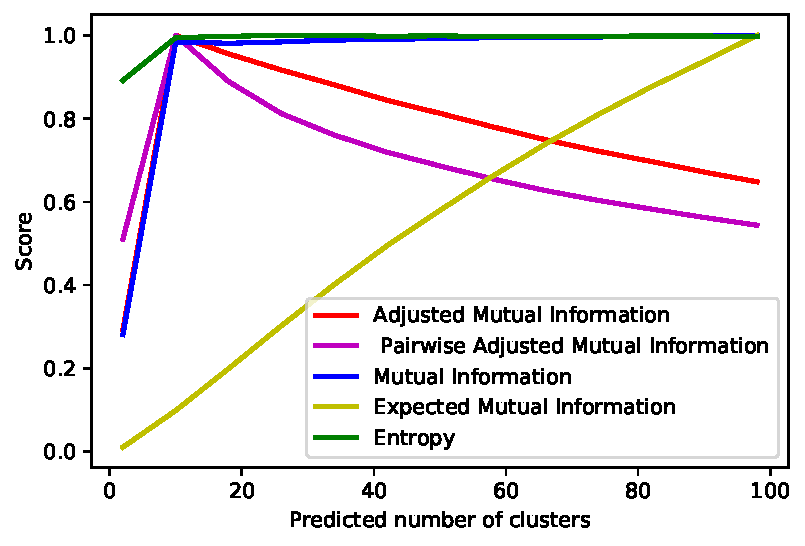
\includegraphics[width=0.5\textwidth]{figures/4-kmeans.pdf}
		\caption{Evaluation of similarity score results on the Gaussian mixture model with $M=10$ clusters and $n=50$ elements in each of it.}
		\label{fig:k_means}
	\end{center}
\end{figure}

Results in Figure \ref{fig:k_means} clearly show why adjustment against chance plays a crucial role for a correct measurement of information between assignments. It is worth to mention, both mutual information and its adjusted versions correctly identify an optimal number of clusters equals to 10. MI shows score similar to maximum everywhere, despite the growth of parameter $k$. In contrast, AMI and PAMI react correctly to the increase of noise and capture actual "information" between assignments. 

\paragraph{Binary Trees}

This experiment is conducted in the following settings: a binary tree with 100 leaves is generated, and we introduce parameter $k$ - a number of shuffled leaf pairs. Afterwards, we shuffle leaves and measure similarity between the original tree and permuted one. Additionally, the experiment is repeated $n_{repetitions}=5$ times to generalise results better.  

\begin{figure}[H]
	\begin{center}
		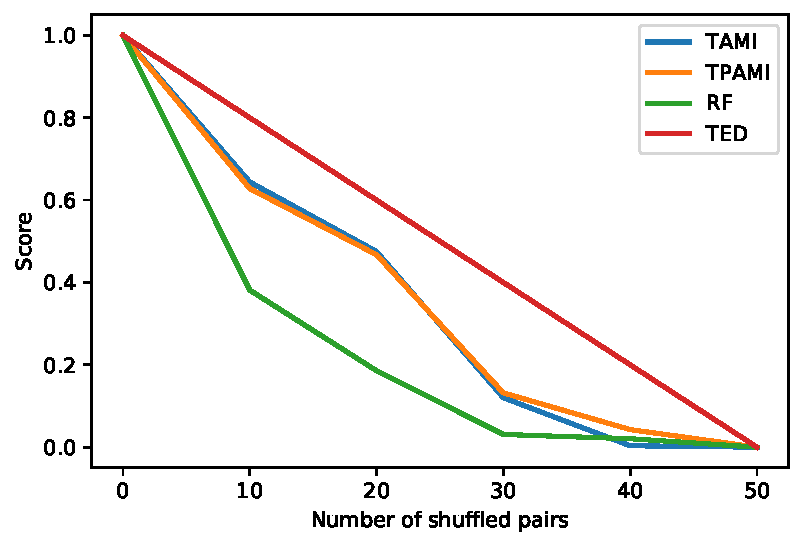
\includegraphics[width=0.5\textwidth]{figures/1-syntatic-trees-binary.pdf}
		\caption{Binary trees with $n=100$ leaves: dependence of the similarity score to the parameter $k$ - shuffled leaf pairs. \label{fig:res}}
		\label{fig:binary_tree_shuffled}
	\end{center}
\end{figure}


\begin{table}[H]
	\begin{center}
		\caption{Binary trees - Pearson correlation between number of shuffled leaf pairs and values of the corresponding metric. \label{binary_corr}}
		\begin{tabular}{rrrr}
\toprule
    TAMI &     TPAMI &        RF &  TED \\
\midrule
-0.96242 & -0.963868 & -0.863864 & -1.0 \\
\bottomrule
\end{tabular}

	\end{center}
\end{table}


Similarity score results can be found in Figure \ref{fig:binary_tree_shuffled}. As we can see, all algorithms capture the trend correctly: with an increasing number of shuffled leaf pairs $k$, the similarity between trees decreases. It is critical to highlight that experiments are conducted on the same tree structure, only leaf names are shuffled. This influences explicitly TED metrics' behaviour, which in this scenario turns into a string-to-string problem and shows perfect performance. Later, we see that it is not the case when tree structure varies.         

To prove quantitatively the statement above, we measure Pearson correlation between metrics' results and noise. Since the noise increases and we expect similarity to decrease it's growth, the correlation is negative see Table \ref{binary_corr}. It demonstrates that the TED metric perfectly correlates with noise, while TAMI and TPAMI have scores around $-0.96$ which is almost exact. RF has the worst performance with the value of $-0.86$.

The run time spent by each metric is depicted in Figure \ref{fig:binary_tree_shuffled_time}. The TED metric clearly has a considerably higher time complexity than others. The time complexities of TAMI and TPAMI are two and six times smaller than those of the TED metric, respectively. 

The following experiment shows how time complexity changes with the number of leaves $n$. We randomly generate a pair of binary trees with $n$ leaves and measure the time needed for the metrics to be calculated. To generalise the results, we repeat the experiment 10 times. 

\begin{itemize}
	\item TED metric has the highest time complexity on relatively small trees Figure \ref{fig:binary_tree_shuffled_time_to_n_leaves_}.  As explained in Chapter \ref{related}, it depends on the number of leaves and each tree's depth. Tree depth equals $log(n)$ for binary trees, which results in high complexity. 
	\item While TAMI is significantly faster in comparison to TED, it is one order slower than TPAMI Figure \ref{fig:binary_tree_shuffled_time_to_n_leaves_zoom}.
	\item TPAMI and RF metrics have similar performance. 
\end{itemize}

\begin{figure}[H]
	\begin{center}
		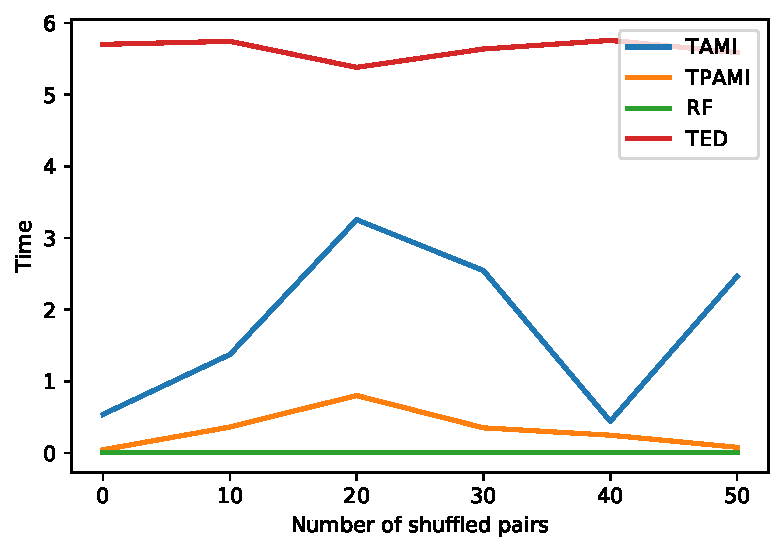
\includegraphics[width=0.5\textwidth]{figures/1-syntatic-time-trees-binary.pdf}
		\caption{Binary trees with $n=100$ leaves: dependence of the time complexity to the parameter $k$ - shuffled leaf pairs.}
		\label{fig:binary_tree_shuffled_time}
	\end{center}
\end{figure}

\begin{figure}[H]
	\centering
	\subfigure{
		\centering
		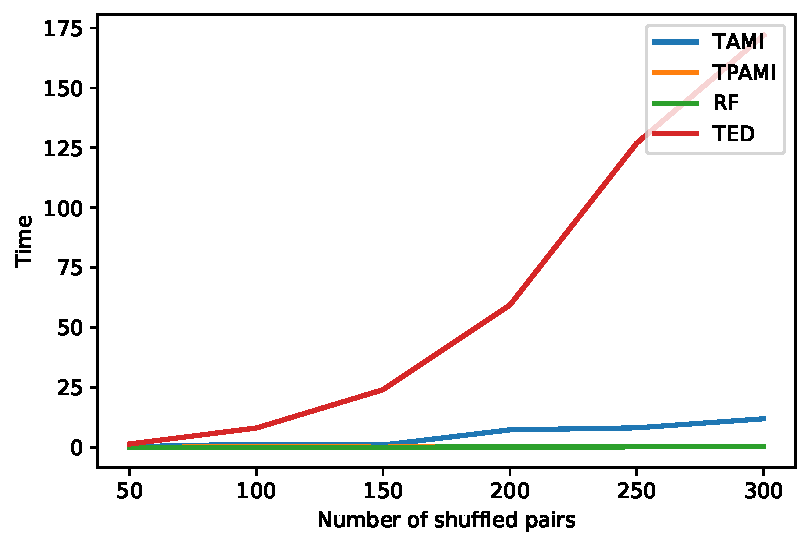
\includegraphics[width=0.46\textwidth]{figures/1-syntatic-binary-tree-time-vs-n-leaves.pdf}
		\label{fig:binary_tree_shuffled_time_to_n_leaves_}
	}
	\subfigure{
		\centering
		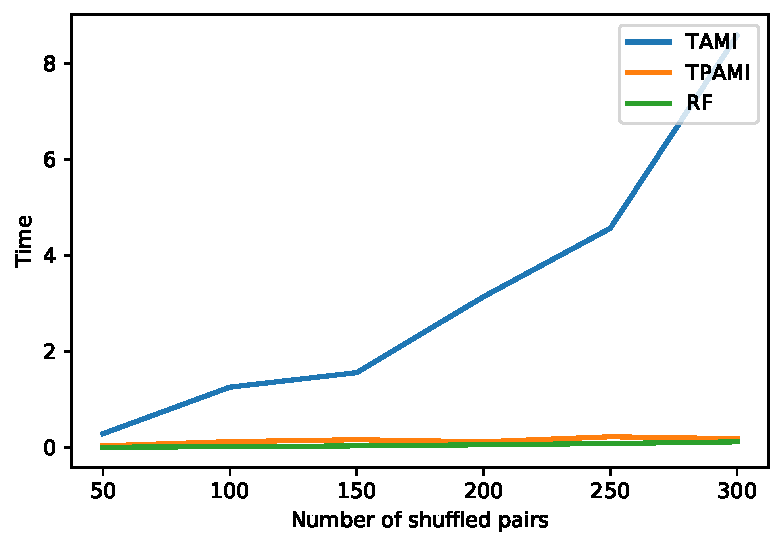
\includegraphics[width=0.46\textwidth]{figures/1-syntatic-binary-tree-time-vs-n-leaves-zoom.pdf}
		\label{fig:binary_tree_shuffled_time_to_n_leaves_zoom}
	}
	\caption{Time complexity between two randomly generated binary trees depending on the number of leaves $n$.}
	\label{fig:binary_tree_shuffled_time_to_n_leaves}
\end{figure}

\paragraph{General Trees}

This is a similar experiment, but instead of binary trees, general trees are considered. 

\begin{figure}[H]
	\begin{center}
		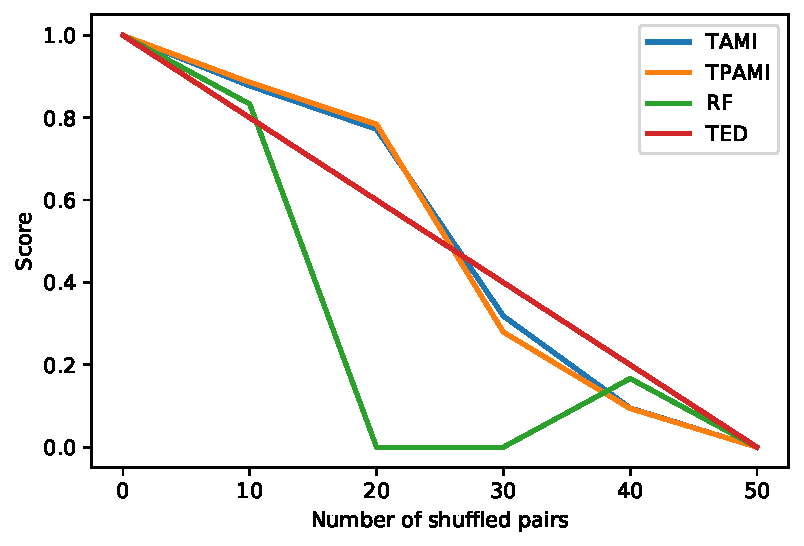
\includegraphics[width=0.5\textwidth]{figures/1-syntatic-trees-general.pdf}
		\caption{General trees with $n=100$ leaves: dependence of the similarity score to the parameter $k$ - shuffled leaf pairs.}
		\label{fig:general_tree_shuffled}
	\end{center}
\end{figure}

\begin{table}[H]
	\begin{center}
		\caption{General trees - Pearson correlation between number of shuffled leaf pairs and values of the corresponding metric. \label{general_corr}}
		\begin{tabular}{rrrr}
\toprule
    TAMI &     TPAMI &        RF &  TED \\
\midrule
-0.97592 & -0.970041 & -0.814345 & -1.0 \\
\bottomrule
\end{tabular}

	\end{center}
\end{table}

Results from Figure \ref{fig:general_tree_shuffled} and Table \ref{general_corr} gives us the following insights:

\begin{itemize}
	\item TED, TAMI, and TPAMI metrics show high correlation scores, meaning that similarity consistently decreases with the growing number of permutations.
	\item In contrast to binary experiment, RF metric does not behave coherently: it drops to 0 with a small amount of noise and jumps when the number of permutations increases. Overall, its performance is unstable, indicating that RF fails to capture dependency between the original tree and the tree with noise. 
\end{itemize}

\begin{figure}[H]
	\begin{center}
		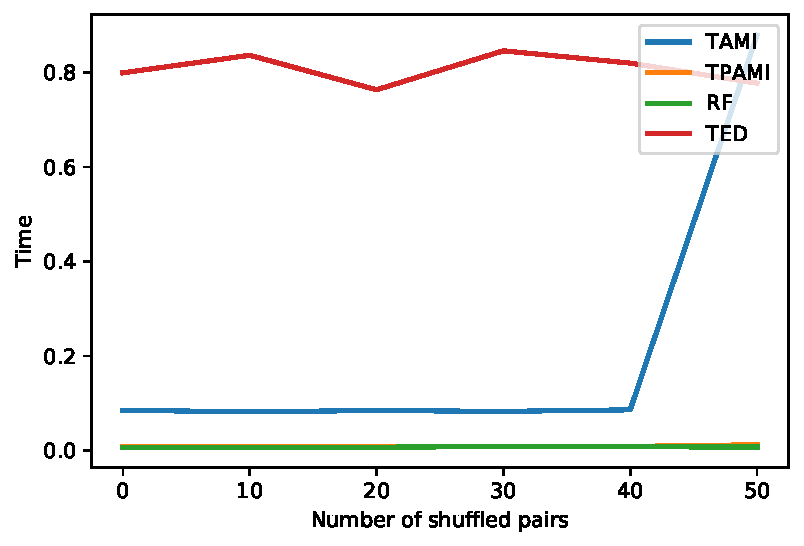
\includegraphics[width=0.5\textwidth]{figures/1-syntatic-time-trees-general.pdf}
		\caption{General trees with $n=100$ leaves: dependence of the time complexity to the parameter $k$ - shuffled leaf pairs.}
		\label{fig:general_tree_shuffled_time}
	\end{center}
\end{figure}

\begin{figure}[H]
	\begin{center}
		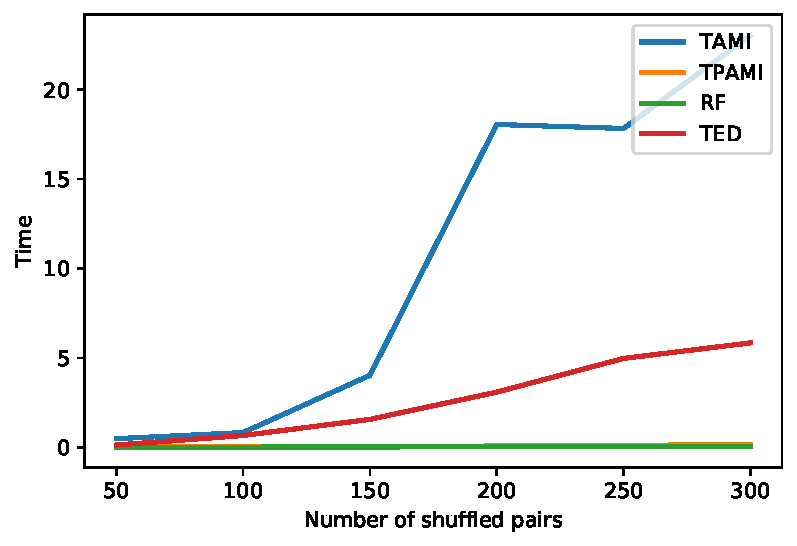
\includegraphics[width=0.5\textwidth]{figures/1-syntatic-general-tree-time-vs-n-leaves.pdf}
		\caption{Time complexity between two randomly generated general trees depending on the number of leaves $n$.}
		\label{fig:general_tree_shuffled_time_to_n_leaves}
	\end{center}
\end{figure}

Time complexity results show us the following:

\begin{itemize}
	\item All metrics have lower time complexities on general trees Figure \ref{fig:general_tree_shuffled_time_to_n_leaves} when compared to binary trees Figure \ref{fig:binary_tree_shuffled_time_to_n_leaves} .
	\item TAMI has the highest complexity and proves its theoretic estimation of $O(n^{2.5})$.
	\item Due to lower tree depth of general trees, time complexity for TED is better than in previous experiment and outperforms that of TAMI.  
	\item TPAMI and RF have the lowest complexities in comparison to others.
\end{itemize}

\paragraph{Stohastic Block Model}
\label{experiment_sbm}

The Stochastic Block Model (SBM) is a generative model that produces graphs with communities. The SBM creates graphs with $n$ nodes $1 \dots n$ that are grouped into $k$ sets $\{C_k, \dots, C_k\}$.
These graphs are generated from a symmetric matrix of edge probabilities $P = \{P_{rs} \}_{1\leq r,s \leq k}$. A unitary weight with probability $P_{rs}$ binds the nodes $i \in C_r$ and $j \in C_s$. 

\begin{figure}[H]
	\begin{center}
		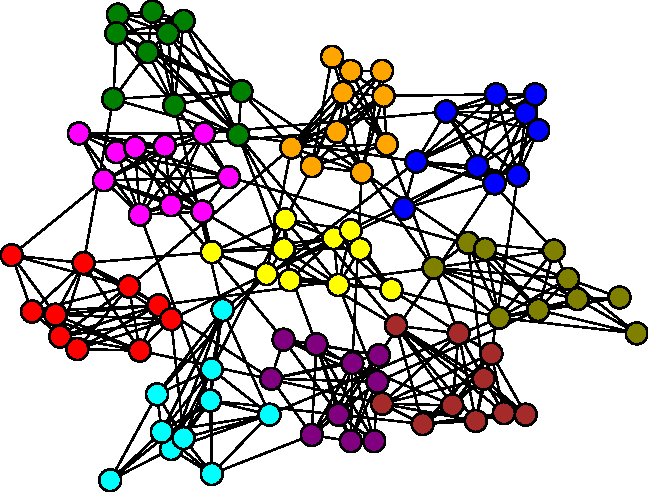
\includegraphics[width=0.65\textwidth]{figures/2-block-model-sbm-graph.pdf}
		\caption{SBM graph with $n=100$ nodes, $p_{in}=1$, $p_{out}=0.01$ and $K=10$ classes which are uniformly distributed. There are 381 edges with an avarage degree of 7.62.}
		\label{fig:sbm_graph}
	\end{center}
\end{figure}

We want to apply hierarchical clustering algorithms discussed earlier in Section \ref{clustering_algorithms} and show how TMI can detect tree similarity with an increasing amount of noise. Firstly, we generate a graph $G_{origin}$ with $n=100$ nodes and $K=10$ clusters with $p_{in}=1$ probability of having edges inside the community and $p_{out}=0.01$ to connect to other clusters. The resulting graph, has 381 edges and an average degree of 7.62. Visualisation can be found in Figure \ref{fig:sbm_graph}. Then we construct a ground truth hierarchy of the given graph represented as a dendrogram $D_{origin}$, which for simplicity only has one level and 10 clusters with 10 nodes in each of them. After applying clustering algorithms: Ward, Louvain and Paris to the graph $G_{origin}$, hierarchies of different qualities are obtained Figure \ref{fig:sbm_dendeogram}. We measure similarity between dendrograms produced by these algorithms and the ground truth hierarchy using metrics discussed in Chapter \ref{related}. We add noise $p_{shuffled}$ by randomly shuffling edges between nodes in the original graph $G_{origin}$, which turns it into a shuffled graph $G_{shuffled}$. The higher the noise, the more difference between dendrograms $D_{origin}$ and $D_{shuffled}$. In order to achieve better generalisation, the experiment is repeated $n_{repetitions}=5$ times. 

\begin{figure}[h]
	\centering
	\subfigure[Ground-truth dendrogram.]{
		\centering
		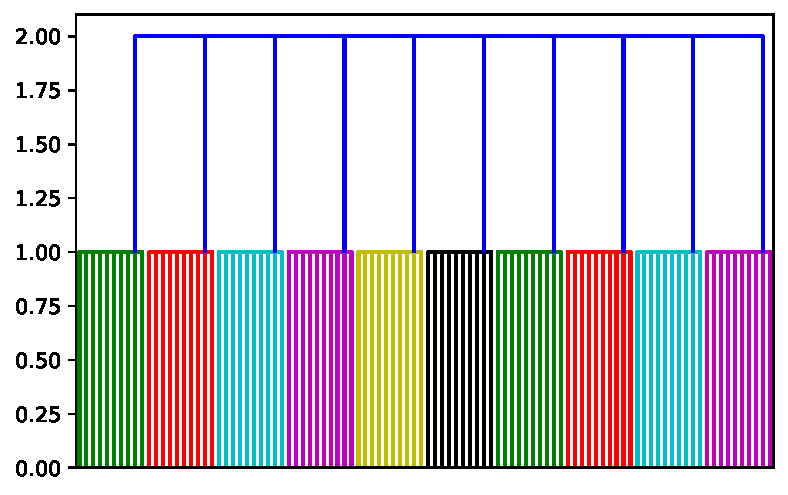
\includegraphics[width=0.46\textwidth,keepaspectratio=true]{figures/2-block-model-sbm-dendrogram_ground_truth.pdf}
		\label{fig:sbm_dendeogram_original}
	}
	\subfigure[Dendrogram obrained after applying the Ward algorithm.]{
		\centering
		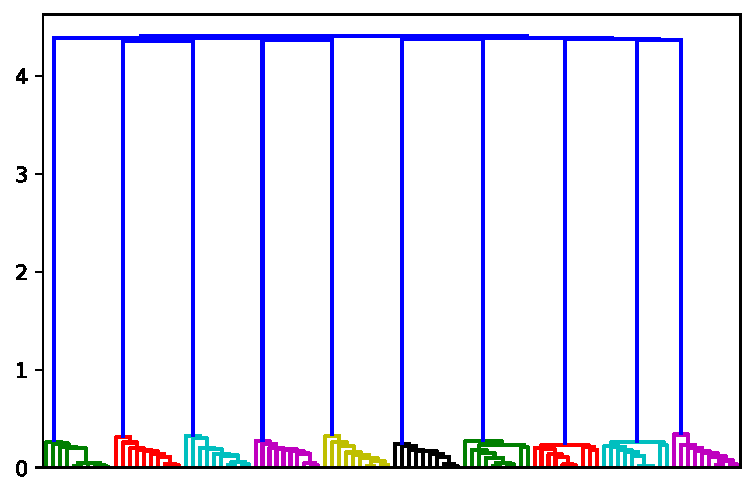
\includegraphics[width=0.46\textwidth,keepaspectratio=true]{figures/2-block-model-sbm-dendrogram_Ward.pdf}
		\label{fig:sbm_dendeogram_ward_}
	}
	\subfigure[Dendrogram obrained after applying the Louvain algorithm.]{
		\centering
		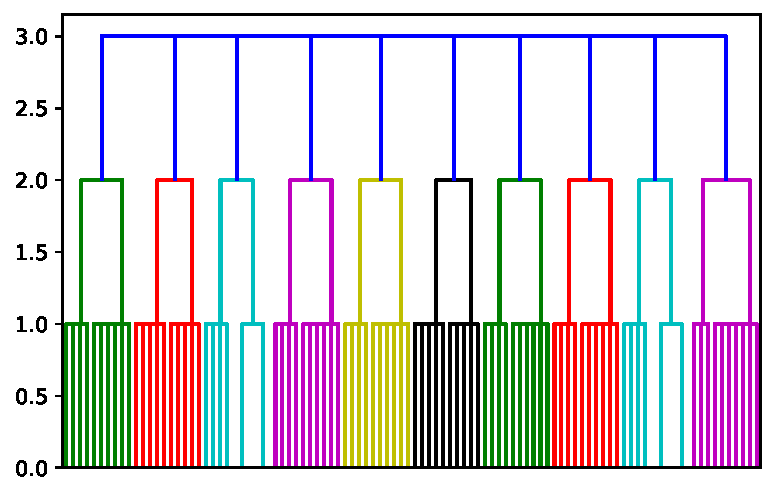
\includegraphics[width=0.46\textwidth,keepaspectratio=true]{figures/2-block-model-sbm-dendrogram_Louvain.pdf}
		\label{fig:sbm_dendeogram_louvain_}
	}
	\subfigure[Dendrogram obrained after applying the Paris algorithm.]{
		\centering
		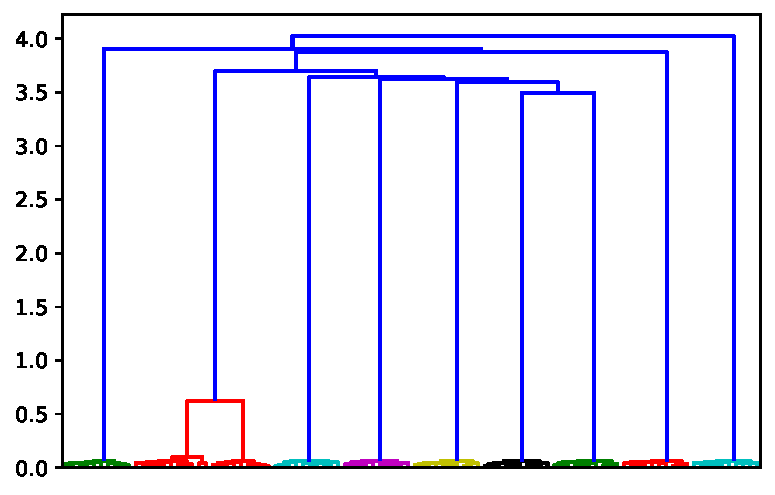
\includegraphics[width=0.46\textwidth,keepaspectratio=true]{figures/2-block-model-sbm-dendrogram_Paris.pdf}
		\label{fig:sbm_dendeogram_paris_}
	}
	\caption{Dendrogram \ref{fig:sbm_dendeogram_original} is syntactically generated, while \ref{fig:sbm_dendeogram_ward_}, \ref{fig:sbm_dendeogram_louvain_}, \ref{fig:sbm_dendeogram_paris_} obtained by applying clustering algorithms presented in Chapter \ref{clustering_algorithms} to the SBM graph.}
	\label{fig:sbm_dendeogram}
\end{figure}

Figure \ref{fig:sbm_results} shows similarity scores between a ground truth dendrogram for the SBM graph and shuffled one obtained using each algorithm: Ward, Louvain and Paris. Results are scaled to lay in the range [0,1].

\begin{itemize}
	\item TPAMI has the best performance in terms of Pearson correlation see Table \ref{sbm_corr}.
	\item TMI with AMI and PAMI behaves very similarly in all experiments and outperforms two other metrics. There is high similarity between the ground truth tree and the one produced by different hierarchical algorithms when the amount of noise is low. When the amount of noise in shuffled graphs increases, similarity gradually decreases. It shows that the newly proposed metric works well with both AMI and PAMI. These functions behave smoothly and coherently. 
	\item In contrast, RF and TED behave very differently depending on the algorithm, which resembles correlation Table \ref{sbm_corr}: both metrics show an unstable performance from one algorithm to another. For example, with the Ward clustering algorithm \ref{fig:sbm_ward}, they can capture similarity with a little amount of noise, but when noise reaches the point $p_{shuffle}=0.4$ both metrics drop to values around 0. For the Louvain algorithm \ref{fig:sbm_louvain} Tree Edited Distance shows very high similarity even with a high amount of noise. By using the Paris clustering algorithm, the final results \ref{fig:sbm_paris} are very unstable: RF and TED almost always show 0 similarity everywhere except for a few spikes.
\end{itemize}

In terms of time performance, we have the following results Figure \ref{fig:sbm_results_time}:

\begin{itemize}
	\item TPAMI faster than TED and TAMI by a factor of 4 and 8 respectively.
	\item TAMI has the worst runtime results. 
\end{itemize} 

\begin{figure}[H]
	\centering
	\subfigure[Similarity results on the Ward dendrogram.]{
		\centering
		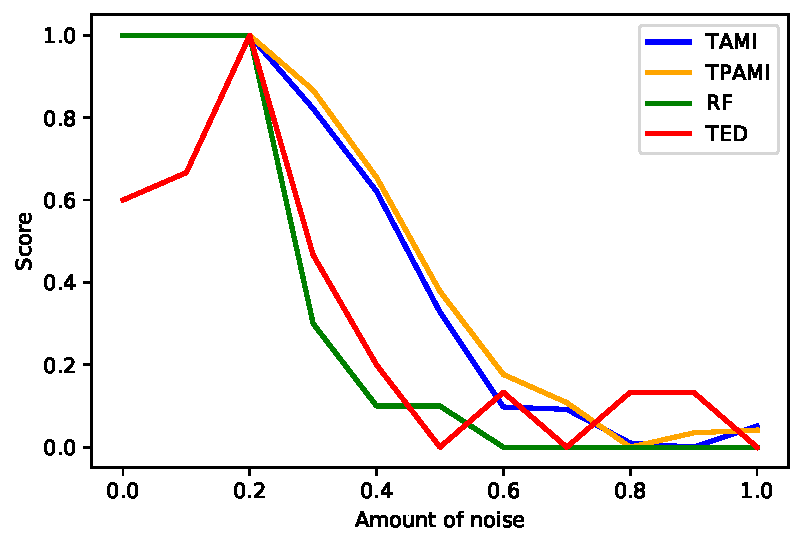
\includegraphics[width=0.46\textwidth, keepaspectratio=true]{figures/2-block-model-sbm-Ward.pdf}
		\label{fig:sbm_ward}
	}
	\subfigure[Similarity results on the Louvain dendrogram.]{
		\centering
		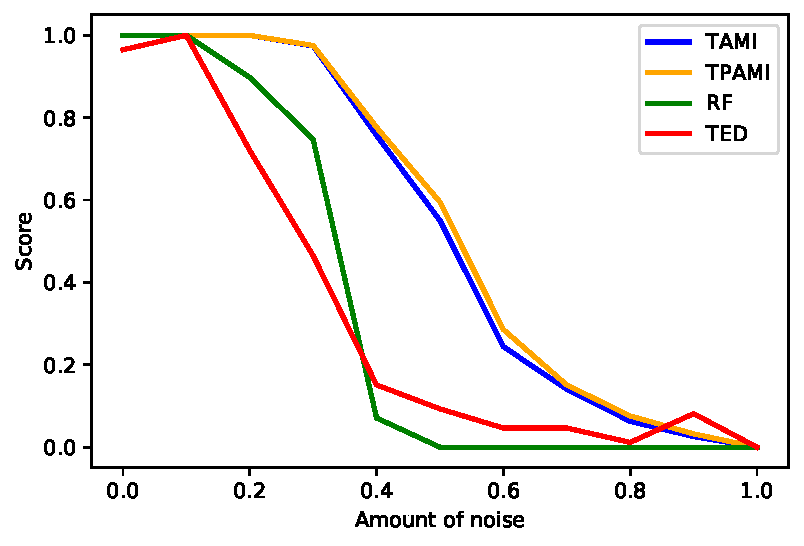
\includegraphics[width=0.46\textwidth, keepaspectratio=true]{figures/2-block-model-sbm-Louvain.pdf}
		\label{fig:sbm_louvain}
	}
	\subfigure[Similarity results on the Paris dendrogram.]{
		\centering
		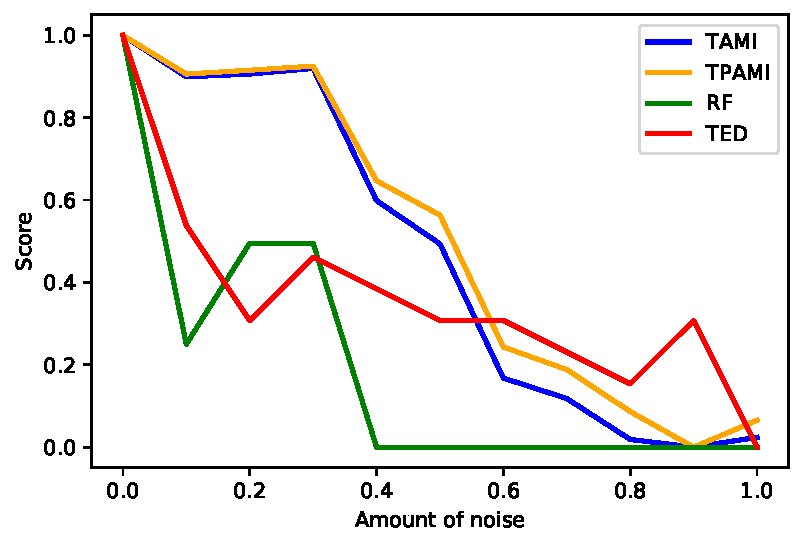
\includegraphics[width=0.46\textwidth, keepaspectratio=true]{figures/2-block-model-sbm-Paris.pdf}
		\label{fig:sbm_paris}
	}
	\caption{Evaluation results on the SBM graph measuring similarity between hierarchies represented by dendrograms $D_{original}$ and $D_{shuffled}$ depending on the amount of noise $p_{shuffled}$.}
	\label{fig:sbm_results}
\end{figure}


\begin{table}[H]
	\begin{center}
		\caption{SBM - Pearson correlation between amount of noise and values of the corresponding metric. \label{sbm_corr}}
		\begin{tabular}{lrrr}
\toprule
{} &      Ward &   Louvain &     Paris \\
\midrule
TAMI  & -0.948200 & -0.961134 & -0.959607 \\
TPAMI & -0.956005 & -0.962542 & -0.964492 \\
RF    & -0.857013 & -0.869449 & -0.771732 \\
TED   & -0.791978 & -0.887756 & -0.817506 \\
\bottomrule
\end{tabular}

	\end{center}
\end{table}

\begin{figure}[H]
	\centering
	\subfigure[Runtime results on the Ward dendrogram.]{
		\centering
		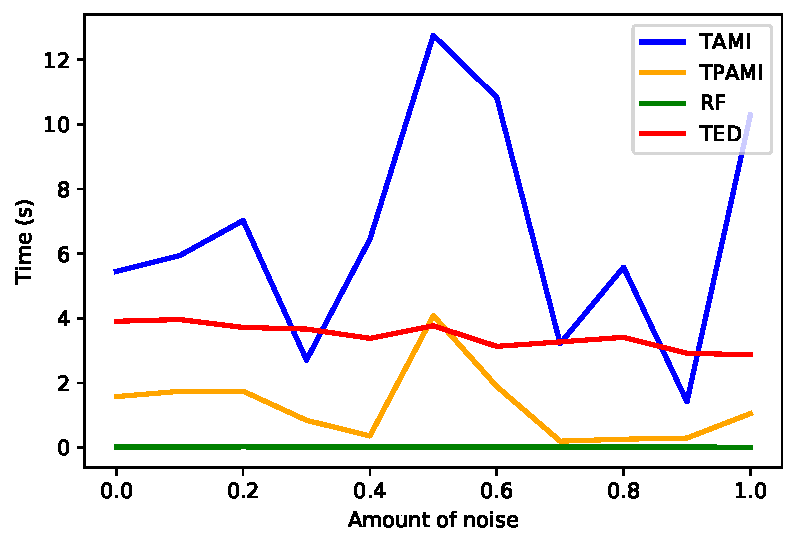
\includegraphics[width=0.46\textwidth, keepaspectratio=true]{figures/2-block-model-sbm-time-Ward.pdf}
		\label{fig:sbm_ward_time}
	}
	\subfigure[Runtime results on the Louvain dendrogram.]{
		\centering
		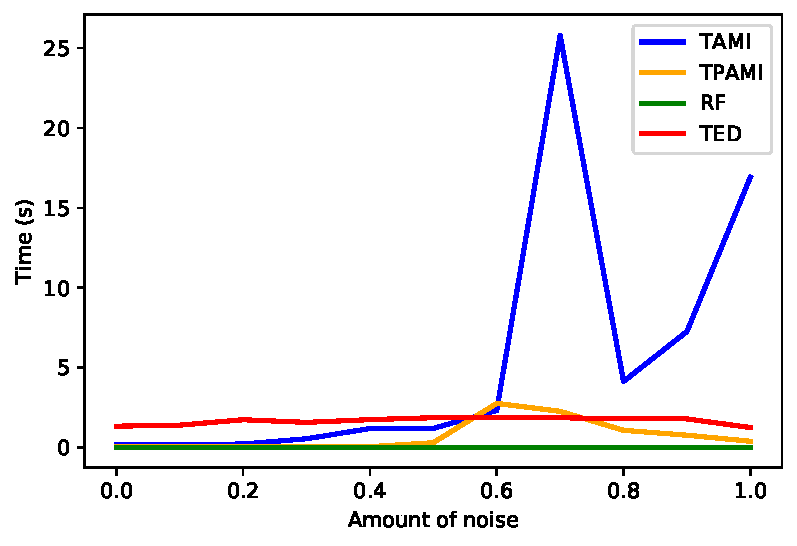
\includegraphics[width=0.46\textwidth, keepaspectratio=true]{figures/2-block-model-sbm-time-Louvain.pdf}
		\label{fig:sbm_louvain_time}
	}
	\subfigure[Runtime results on the Paris dendrogram.]{
		\centering
		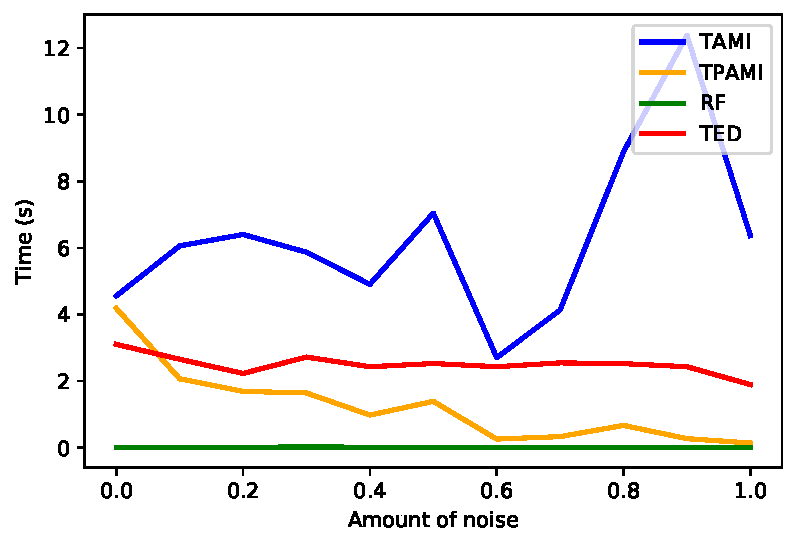
\includegraphics[width=0.46\textwidth, keepaspectratio=true]{figures/2-block-model-sbm-time-Paris.pdf}
		\label{fig:sbm_paris_time}
	}
	\caption{Evaluation results on the SBM graph measuring time complexity of each metric depending on the amount of noise $p_{shuffled}$.}
	\label{fig:sbm_results_time}
\end{figure}


\begin{table}[H]
	\centering
	\caption{Evaluation results on the SBM graph measuring optimal number of clusters between hierarchies represented by dendrograms $D_{original}$ and $D_{shuffled}$ depending on the amount of noise $p_{shuffled}$. Tree Mutual Information with AMI and PAMI metrics are compared. \label{fig:sbm_results_n_clusters}}
	\subfigure[TAMI.]{
		\centering
		\small\addtolength{\tabcolsep}{-6pt}
		\begin{tabular}{llllllllllll}
\toprule
{} &       0.0 &       0.1 &       0.2 &       0.3 &       0.4 &       0.5 &       0.6 &       0.7 &       0.8 &       0.9 &       1.0 \\
\midrule
Ward    &  [10, 10] &  [10, 10] &  [10, 10] &   [10, 8] &   [10, 9] &  [10, 13] &  [46, 24] &  [37, 16] &  [64, 19] &  [37, 11] &  [46, 24] \\
Louvain &  [10, 10] &  [10, 10] &  [10, 10] &  [10, 11] &  [10, 12] &  [10, 12] &  [19, 14] &  [37, 41] &  [28, 21] &  [37, 25] &  [55, 38] \\
Paris   &  [10, 10] &  [10, 10] &  [10, 10] &  [10, 10] &  [19, 10] &   [10, 9] &  [46, 13] &  [37, 16] &  [64, 21] &  [64, 23] &  [64, 23] \\
\bottomrule
\end{tabular}
 
	}
	\subfigure[TPAMI.]{
		\centering
		\small\addtolength{\tabcolsep}{-6pt}
		\begin{tabular}{llllllllllll}
\toprule
{} &       0.0 &       0.1 &       0.2 &       0.3 &       0.4 &       0.5 &       0.6 &       0.7 &       0.8 &       0.9 &       1.0 \\
\midrule
Ward    &  [10, 10] &  [10, 10] &  [10, 10] &   [10, 8] &   [10, 6] &  [10, 13] &  [28, 26] &   [37, 7] &   [46, 8] &  [37, 11] &  [46, 20] \\
Louvain &  [10, 10] &  [10, 10] &  [10, 10] &   [10, 9] &   [10, 8] &  [10, 12] &  [10, 21] &  [37, 36] &  [37, 30] &  [37, 24] &  [46, 23] \\
Paris   &  [10, 10] &  [10, 10] &  [10, 10] &  [10, 10] &  [19, 10] &   [10, 9] &  [46, 10] &  [37, 11] &  [55, 15] &   [55, 2] &   [55, 9] \\
\bottomrule
\end{tabular}

	}
\end{table}

\newpage

By analysing optimal number of clusters in Table \ref{fig:sbm_results_n_clusters} we see that: 
\begin{itemize}
	\item TAMI and TPAMI identify the optimal number of clusters correctly when the amount of noise is less than 0.3.
	\item With noise in a range of [0.3, 0.5] depending on algorithms metrics also shows a relatively correct number of clusters: for Ward, we see 10 vs 9 or 8 while for Louvain, it is 10 vs 12 or 11.
	\item When $p_{shuffled} > 0.5$, fluctuation in the optimal number of clusters is quite significant for both metrics.
	\item It is worth mentioning that TPAMI tends to show the smaller number and stop earlier without going too deep into a tree structure in contrast to the TAMI metric. This also highly correlates with time spent by each metric \ref{fig:sbm_results_time}: TPAMI is significantly faster than the TAMI metric. 
\end{itemize} 


\paragraph{Hierarchical Stochastic Block Model}

\begin{figure}[H]
	\centering
	\subfigure[Ground-truth.]{
		\centering
		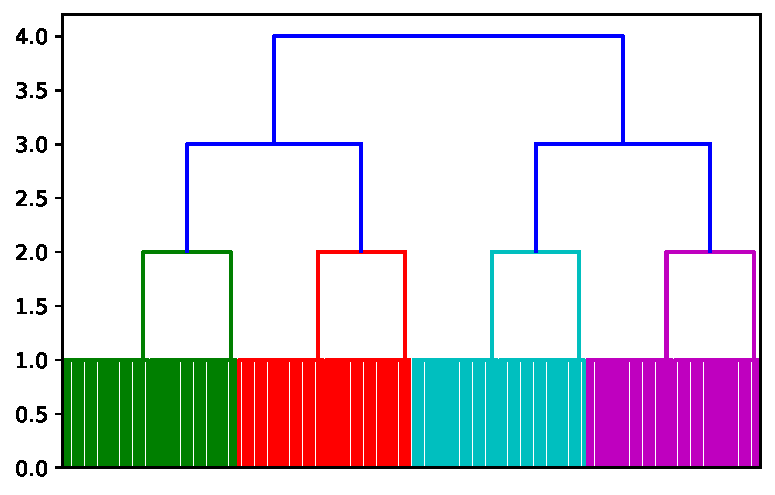
\includegraphics[width=0.46\textwidth,keepaspectratio=true]{figures/2-block-model-hsbm-dendrogram_ground_truth.pdf}
		\label{fig:hsbm_dendeogram_original}
	}
	\subfigure[Ward.]{
		\centering
		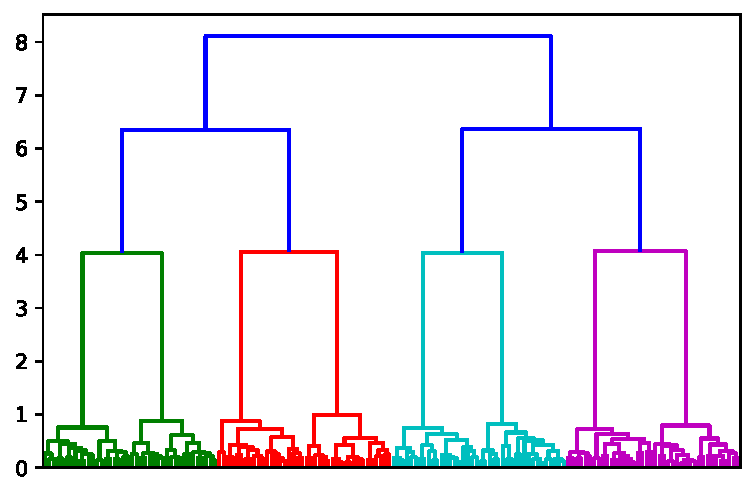
\includegraphics[width=0.46\textwidth,keepaspectratio=true]{figures/2-block-model-hsbm-dendrogram_Ward.pdf}
		\label{fig:hsbm_dendeogram_ward}
	}
	\subfigure[Louvain.]{
		\centering
		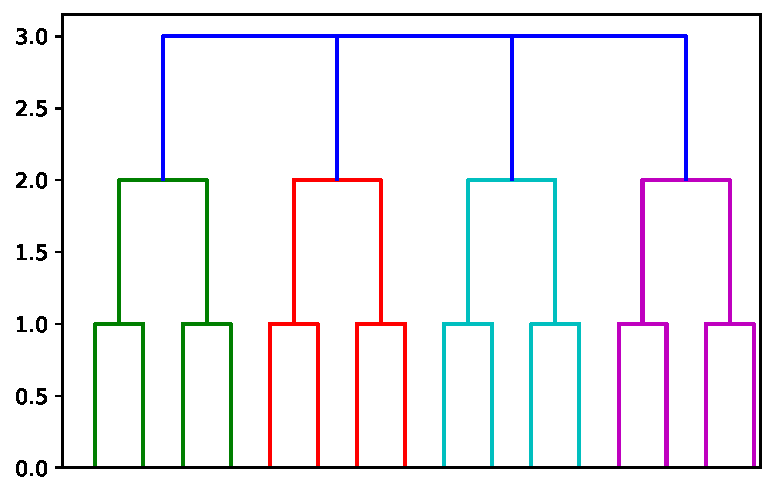
\includegraphics[width=0.46\textwidth,keepaspectratio=true]{figures/2-block-model-hsbm-dendrogram_Louvain.pdf}
		\label{fig:hsbm_dendeogram_louvain}
	}
	\subfigure[Paris.]{
		\centering
		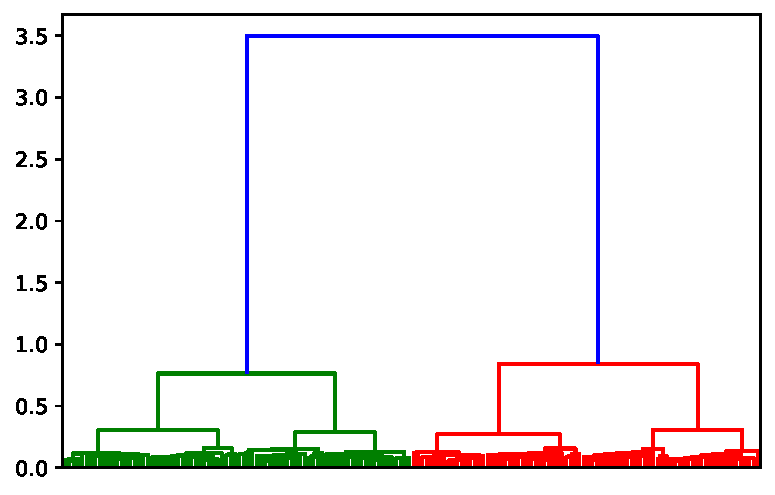
\includegraphics[width=0.46\textwidth,keepaspectratio=true]{figures/2-block-model-hsbm-dendrogram_Paris.pdf}
		\label{fig:hsbm_dendeogram_paris}
	}
	\caption{Dendrogram \ref{fig:hsbm_dendeogram_original} is syntactically generated, while \ref{fig:hsbm_dendeogram_ward}, \ref{fig:hsbm_dendeogram_louvain}, \ref{fig:hsbm_dendeogram_paris} obtained by applying clustering algorithms \ref{clustering_algorithms} to the HSBM graph.}
	\label{fig:hsbm_dendeogram}
\end{figure}

While it is effective to construct communities, the SBM \ref{experiment_sbm} lacks a clear way to produce graphs with hierarchies. Furthermore, actual graphs often tend to have several relevant clustering scales, which motivates the concept of a hierarchical variant of SBM, as discussed in \cite{charpentier2019master} and \cite{lyzinski2016community}. In this experiment, we consider a hierarchical stochastic block model (HSBM) with Poisson distributed edge weights of 160 nodes and 3 levels of hierarchy (a binary tree with leaves corresponding to clusters of 20 nodes) with parameters: $decay\_factor=0.3$, $p_{in}=0.9$. The resulted graph has 2223 edges with an average degree of 27.6. The other settings for the experiment are the same as for \ref{experiment_sbm}. Visualisation of dendrograms can be seen in Figure \ref{fig:hsbm_dendeogram}.


\begin{figure}[H]
	\centering
	\subfigure[Ward.]
	{
		\centering
		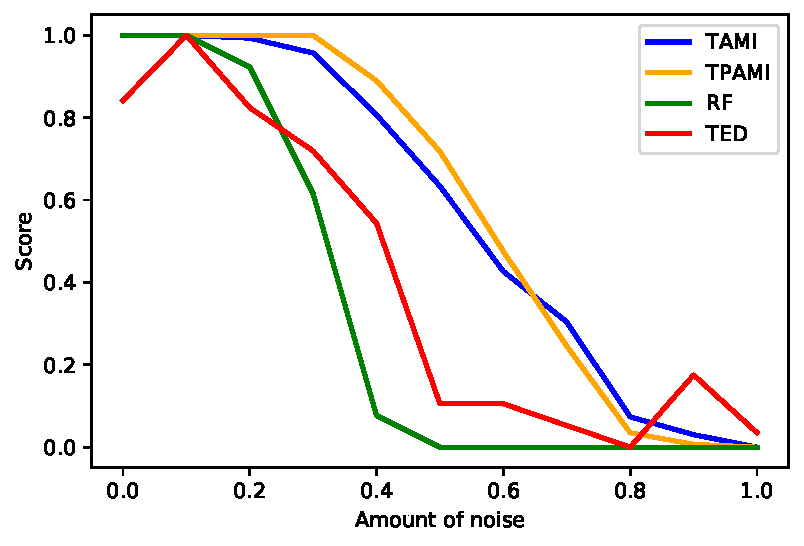
\includegraphics[width=0.46\textwidth,keepaspectratio=true]{figures/2-block-model-hsbm-Ward.pdf}
	}
	\subfigure[Louvain.]{
		\centering
		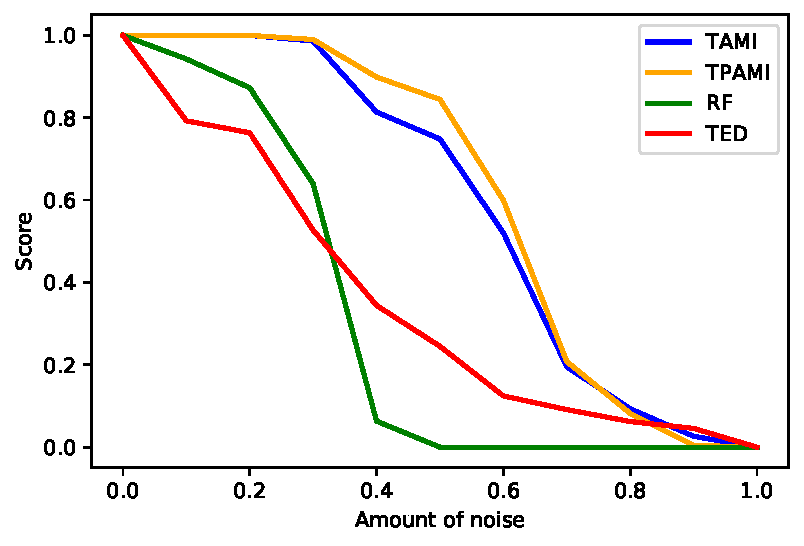
\includegraphics[width=0.46\textwidth,keepaspectratio=true]{figures/2-block-model-hsbm-Louvain.pdf}
	}
	\subfigure[Paris.]{
		\centering
		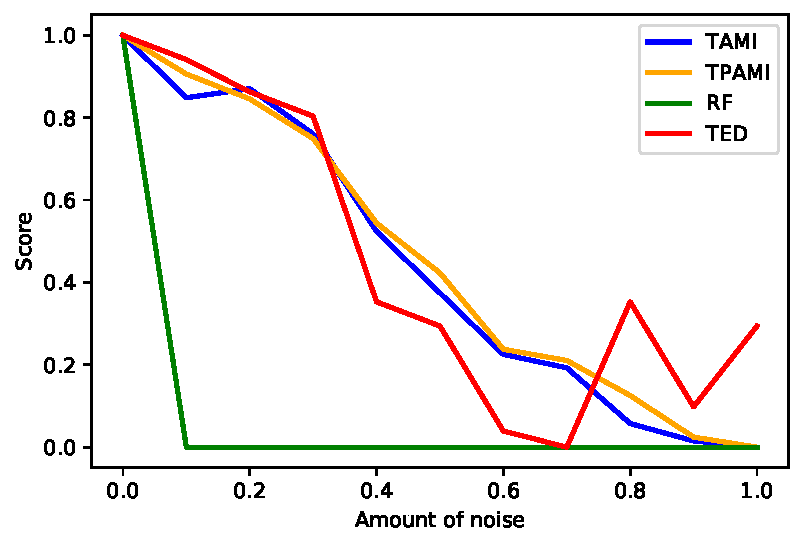
\includegraphics[width=0.46\textwidth,keepaspectratio=true]{figures/2-block-model-hsbm-Paris.pdf}
		\label{fig:hsbm_paris}
	}
	\caption{Evaluation results on HSBM graph measuring similarity between hierarchies represented by dendrograms $D_{original}$ and $D_{shuffled}$ depending on the amount of noise $p_{shuffled}$.}
	\label{fig:hsbm_results}
\end{figure}


\begin{table}[H]
	\begin{center}
		\caption{HSBM - Pearson correlation between amount of noise and values of the corresponding metric. \label{hsbm_corr}}
		\begin{tabular}{lrrr}
\toprule
{} &      Ward &   Louvain &     Paris \\
\midrule
TAMI  & -0.970748 & -0.956428 & -0.981013 \\
TPAMI & -0.952583 & -0.936338 & -0.988256 \\
RF    & -0.871165 & -0.871952 & -0.500000 \\
TED   & -0.904393 & -0.955369 & -0.809923 \\
\bottomrule
\end{tabular}

	\end{center}
\end{table}


The outcomes Figure \ref{fig:hsbm_results} and Table \ref{hsbm_corr} of the HSBM experiment resemble behaviour which was seen on SBM: 

\begin{itemize}
	\item Tree Mutual Information with AMI and PAMI performs much better than RF and TED. TAMI and TPAMI show correlation that is almost equal to 1.
	\item Unstable behaviour using Paris algorithm is seen for RF and TED: RF almost always shows 0 similarity score while TED has stepped view with the a very abrupt decline to 0 and little spikes at the end. Pearson correlation for the RF metric shows results in a range from -0.87 to -0.5, which is poor.
\end{itemize} 


\begin{figure}[H]
	\centering
	\subfigure[Runtime results on the Ward dendrogram.]{
		\centering
		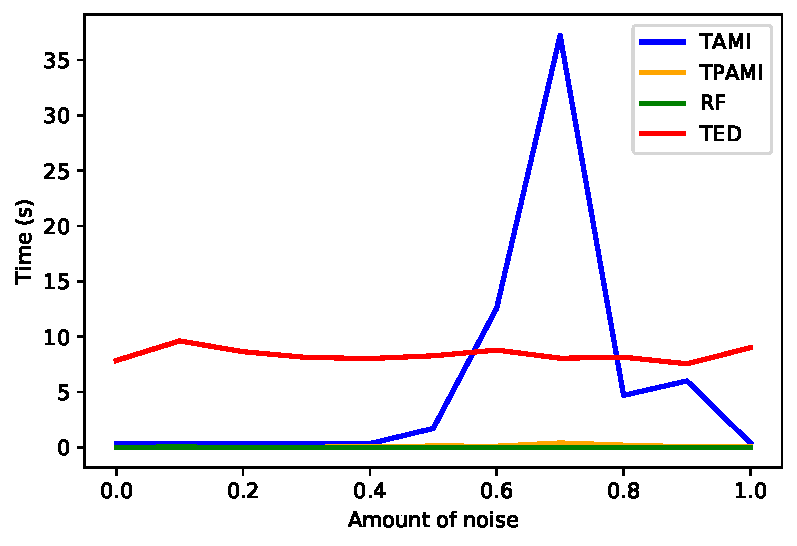
\includegraphics[width=0.46\textwidth,keepaspectratio=true]{figures/2-block-model-hsbm-time-Ward.pdf}
		\label{fig:hsbm_ward_time}
	}
	\subfigure[Runtime results on the Louvain dendrogram.]{
		\centering
		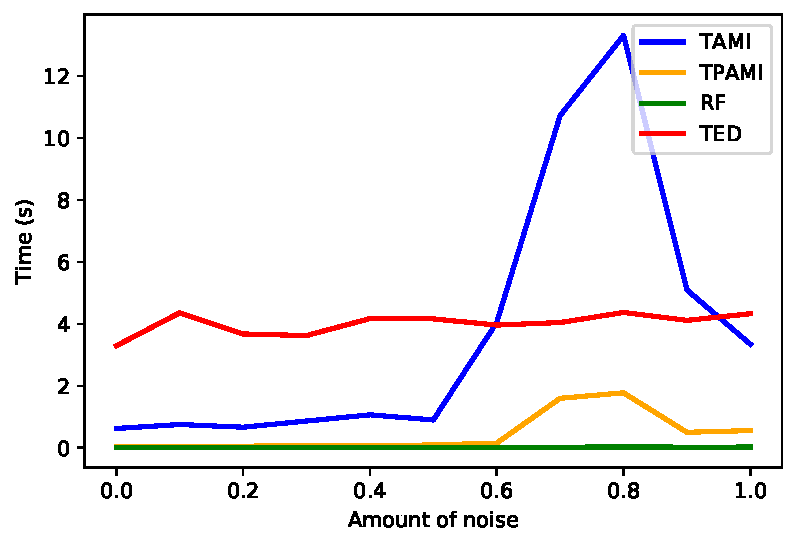
\includegraphics[width=0.46\textwidth,keepaspectratio=true]{figures/2-block-model-hsbm-time-Louvain.pdf}
		\label{fig:hsbm_louvain_time}
	}
	\subfigure[Runtime results on the Paris dendrogram.]{
		\centering
		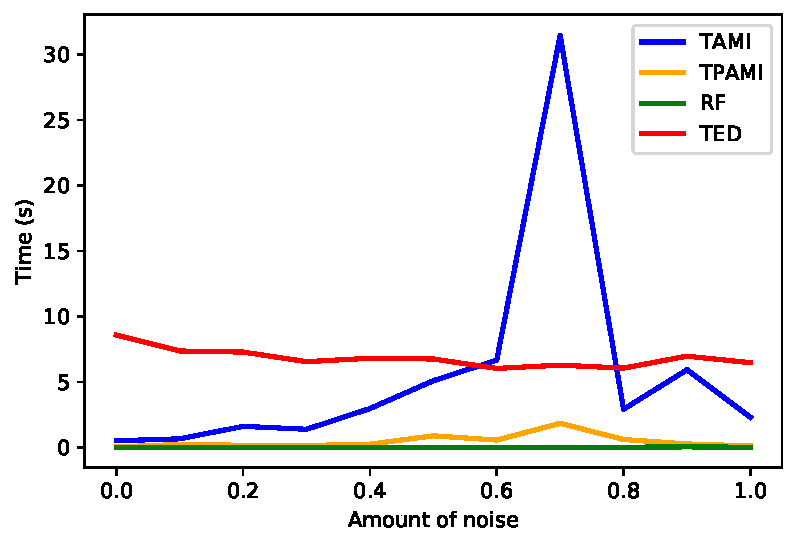
\includegraphics[width=0.46\textwidth,keepaspectratio=true]{figures/2-block-model-hsbm-time-Paris.pdf}
		\label{fig:hsbm_paris_time}
	}
	\caption{Evaluation results on HSBM graph measuring time complexity of each metric depending on the amount of noise $p_{shuffled}$.}
	\label{fig:hsbm_results_time}
\end{figure}

Analysing time complexity results from Figure \ref{fig:hsbm_results_time} we can see that TPAMI has nearly as good performance as the RF metric. TAMI has the worst outcomes while TED remains stable over different values on the [0,1]. 


\begin{table}[H]
	\centering
	\caption{Evaluation results on the HSBM graph measuring optimal number of clusters between hierarchies represented by dendrograms $D_{original}$ and $D_{shuffled}$ depending on the amount of noise $p_{shuffled}$. Tree Mutual Information with AMI and PAMI metrics are compared. \label{fig:hsbm_results_n_clusters}}
	\subfigure[TAMI.]{
		\centering
		\small\addtolength{\tabcolsep}{-6pt}
		\begin{tabular}{llllllllllll}
\toprule
{} &     0.0 &     0.1 &      0.2 &      0.3 &      0.4 &      0.5 &       0.6 &       0.7 &       0.8 &       0.9 &       1.0 \\
\midrule
Ward    &  [8, 8] &  [8, 8] &   [8, 8] &   [8, 8] &   [7, 7] &  [6, 12] &  [24, 18] &  [43, 40] &  [33, 21] &  [24, 16] &   [23, 7] \\
Louvain &  [8, 8] &  [8, 8] &   [8, 8] &   [8, 8] &  [8, 11] &  [7, 13] &  [15, 23] &  [26, 41] &  [34, 48] &  [22, 47] &  [13, 29] \\
Paris   &  [8, 9] &  [8, 8] &  [8, 11] &  [8, 11] &  [7, 14] &  [6, 15] &  [25, 16] &  [17, 28] &  [15, 12] &  [23, 21] &  [33, 15] \\
\bottomrule
\end{tabular}
 
	}
	\subfigure[TPAMI.]{
		\centering
		\small\addtolength{\tabcolsep}{-6pt}
		\begin{tabular}{llllllllllll}
\toprule
{} &     0.0 &     0.1 &     0.2 &     0.3 &      0.4 &      0.5 &      0.6 &       0.7 &       0.8 &       0.9 &      1.0 \\
\midrule
Ward    &  [4, 4] &  [4, 4] &  [4, 4] &  [4, 4] &   [5, 5] &   [5, 7] &   [6, 6] &  [15, 12] &  [23, 12] &    [5, 7] &  [23, 7] \\
Louvain &  [4, 4] &  [4, 4] &  [4, 4] &  [5, 5] &   [4, 4] &   [5, 5] &  [5, 16] &  [16, 39] &   [5, 38] &   [3, 31] &  [4, 27] \\
Paris   &  [5, 5] &  [5, 8] &  [6, 8] &  [6, 8] &  [6, 10] &  [6, 14] &  [6, 11] &  [17, 21] &  [16, 16] &  [14, 10] &  [33, 8] \\
\bottomrule
\end{tabular}

	}
\end{table}

In terms of an optimal number of clusters Table \ref{fig:hsbm_results_n_clusters} the case of HSBM is more difficult than SBM. There are different levels of hierarchy in ground-truth dendrogram \ref{fig:hsbm_dendeogram_original}: on the first level, we have 2 clusters which further are subdivided into 2 resulting in 4 clusters. On level 3, we have 8 clusters with 20 nodes each. 

\begin{itemize}
	\item TAMI and TPAMI identify an optimal number of clusters a bit differently: TAMI shows 8 clusters as optimal for Ward and Louvain when the amount of noise is less than 0.5, while TPAMI on the same settings gives 4 as an optimal number.
	\item We can see that TPAMI tends to early stop at level 2 of the ground truth dendrogram from Figure \ref{fig:hsbm_dendeogram_original}. 
	\item However, when $p_{shuffled}$ is bigger than 0.5, fluctuation in the optimal number of clusters is quite significant for both metrics.
	\item It is worth mentioning that TPAMI tends to show smaller numbers and stop earlier without going too deep into a tree structure, in contrast to the TAMI metric. This highly correlates evaluation time of each metric Figure \ref{fig:sbm_results_time}: TPAMI is significantly faster than the TAMI metric. 
	\item The structure of the tree generated using the Paris algorithm is interpreted by both metrics differently than the one generated with Ward and Louvain. We see that TAMI predicts [8,9], while TPAMI predicts [5,5], [5,7] as optimal number of clusters.
\end{itemize} 

These results may indicate that our decision to model the ground-truth dendrogram Figure \ref{fig:hsbm_dendeogram_original} as a binary tree with 20 leaves in 4 levels was wrong. Therefore, we notice this instability during evaluation. This is another very useful feature of our new metric, which can be used not only to test the quality of clustering algorithms but also to check the quality of ground-truth trees/dendrograms.

\section{Real datasets}
As stated in Section \ref{cashing}, we use cashing to speed up the TAMI metric computation on large datasets. To optimise its execution even more, part of the code was written in Cython \cite{behnel2011cython} utilising built-in parallelisation. Additionally, in order to compute the first part of Formula \ref{eq:ami} instead of the NumPy \cite{harris2020array} version of Mutual Information, C based implementation from \cite{feast}. Utilising all these improvements we cut execution time by more than 50 times. 

Next, we show the practical interest of TMI in terms of tree comparison. Experiments on real networks are performed on 2 datasets with various sizes and sparsity. Detailed information about these datasets can be found in Table \ref{datasets_information}. Both datasets are taken from \cite{netset}.

\begin{table}[H]
	\centering
	\caption{Summary of the 2 datasets.}
	\label{openflights_trees_information}
	\begin{tabular}{lrrr}
\toprule
Dataset &  nodes &  edges &  average degree \\
\midrule
OpenFlight  &  3097 &     18193 &   11.74 \\
WikiVitals  &  10012 &    792091 &  158.22 \\
\bottomrule
\end{tabular}

\label{datasets_information}  
\end{table}

We want to compute a similarity matrix $s(A, B)$ for trees obtained with Ward, Paris and Louvain algorithms on Openflights and WikiVitals datasets. The Ward algorithm has a GSVD embedding method with the number of components equal to 20 and regularisation of 0.1; for the Louvain algorithm we set depth equal to 20. We conduct these experiments only with metrics proposed in Chapter \ref{design}. We disregard RF and TED metrics due to bad performance in the clustering scenario and inefficiency when applied to large datasets.  

\paragraph{Openflights}

\begin{figure}[h]
	\caption{OpenFlights graph \cite{netset}.  \label{fig:openflights_graph}}
	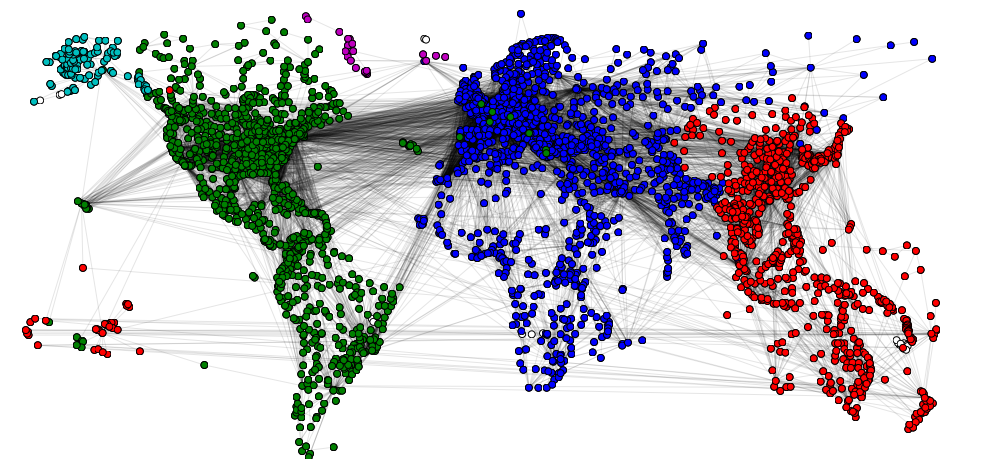
\includegraphics[width=0.65\textwidth,keepaspectratio=true]{figures/openflights_visualization.png}
	\centering
\end{figure}

OpenFlights is a weighted graph in which nodes represent airports worldwide and edge weights represent the number of flights between two airports. They display various regions around the world, like natural visual clusters including continents and countries. 

\begin{table}[h]
	\centering
	\caption{Openflights - trees information. \label{openflight_trees_information}}
	\begin{tabular}{lrrr}
\toprule
{} &  Ward &  Louvain &  Paris \\
\midrule
Number of leaf nodes  &  3097 &     3097 &   3097 \\
Total number of nodes &  6005 &     4274 &   6193 \\
Most distant node     &   237 &     3053 &   1706 \\
Max. distance         &    24 &        7 &     32 \\
\bottomrule
\end{tabular}
    
\end{table}

We apply all three algorithms to the dataset, convert the output to trees and obtain trees with the following statistics seen in Table \ref{openflight_trees_information}. We can see that the structure of these trees is very different: they have distinct numbers of hierarchical layers varying from 7 to 32 and a different total number of nodes. 

\begin{table}[h]
	\centering
	\caption{Openflights - similarity matrix. \label{openflight_similarity}}
	\subfigure[TAMI.]{
		\centering
		\begin{tabular}{lrrr}
\toprule
{} &  Ward &  Paris &  Louvain \\
\midrule
Ward    &  3.38 &   2.41 &     2.40 \\
Paris   &  2.41 &   3.36 &     2.64 \\
Louvain &  2.40 &   2.64 &     3.27 \\
\bottomrule
\end{tabular}
 
		\label{openflight_similarity_tami}
	}
	\subfigure[TPAMI.]{
		\begin{tabular}{llll}
\toprule
{} &  Ward & Paris & Louvain \\
\midrule
Ward    &     3 &  2.26 &    2.22 \\
Paris   &  2.26 &  2.98 &     2.4 \\
Louvain &  2.22 &   2.4 &    2.87 \\
\bottomrule
\end{tabular}

		\label{openflight_similarity_tpami}
	}
\end{table}

We compare all these dendrograms with each other, and the results can be found in Table \ref{openflight_similarity}. We can see that TAMI Table \ref{openflight_similarity_tami} and TPAMI Table \ref{openflight_similarity_tpami} identify the same similarity order between trees. For example, for the Ward tree both metrics show that the highest similarity is obtained with the identical tree, then the tree obtained by applying Paris algorithm which is more similar than Louvain. As was mentioned in Chapter \ref{design}, magnitude can vary because, we do not use normalisation. 

\begin{table}[h]
	\centering
	\caption{Openflights - optimal number of clusters.   \label{openflight_n_clusters}}
	\subfigure[TAMI.]{
		\centering
		\begin{tabular}{llll}
\toprule
{} &       Ward &     Paris &    Louvain \\
\midrule
Ward    &    (64-64) &   (94-68) &  (120-149) \\
Paris   &    (68-94) &   (65-65) &   (82-130) \\
Louvain &  (149-120) &  (130-82) &    (93-93) \\
\bottomrule
\end{tabular}
 
	}
	\subfigure[TPAMI.]{
		\begin{tabular}{llll}
\toprule
{} &      Ward &     Paris &   Louvain \\
\midrule
Ward    &    (7, 7) &  (48, 38) &  (67, 72) \\
Paris   &  (38, 48) &  (11, 11) &  (25, 47) \\
Louvain &  (72, 67) &  (47, 25) &  (35, 35) \\
\bottomrule
\end{tabular}

	}
\end{table}

In Table \ref{openflight_n_clusters} we see the optimal number of clusters for each pair of trees. We observe behaviour to previous experiments: TPAMI tends to identify fewer clusters and stops earlier than TAMI. 

\begin{table}[h]
	\centering
	\caption{Openflights - time complexities (s). \label{openflight_time}}
	\subfigure[TAMI.]{
		\centering
		\begin{tabular}{lrrr}
\toprule
{} &  Ward &  Paris &  Louvain \\
\midrule
Ward    &    17 &     94 &      598 \\
Paris   &    94 &     20 &     1142 \\
Louvain &   598 &   1142 &        6 \\
\bottomrule
\end{tabular}
 
	}
	\subfigure[TPAMI.]{
		\begin{tabular}{llll}
\toprule
{} & Ward & Paris & Louvain \\
\midrule
Ward    &    1 &    43 &     111 \\
Paris   &   43 &     3 &      48 \\
Louvain &  111 &    48 &       2 \\
\bottomrule
\end{tabular}

	}
\end{table}

Table \ref{openflight_time} presents time complexities of the experiment. TPAMI works much faster than the TAMI metric due to its lower complexity by construction and early stopping property.

\paragraph{Wikivitals}

The Wikivitals dataset is an unweighted graph where nodes represent Vital articles of Wikipedia with links between them and words used in summaries. We reconstruct the hierarchy from ground truth labels: there are 4 levels with the following number of clusters on each: 11, 109, 491, 1164. We convert the ground truth dendrogram into a tree and consider it  as an additional tree in the experiment. 

\begin{table}[h]
	\centering
	\caption{Wikivitals - trees information. \label{wikivitals_trees_information}}
	\begin{tabular}{lrrrr}
\toprule
{} &  Ground Truth &   Ward &  Louvain &  Paris \\
\midrule
Number of leaf nodes  &         10012 &  10012 &    10012 &  10012 \\
Total number of nodes &         11319 &  20023 &    14231 &  20023 \\
Most distant node     &         10011 &   4924 &     9516 &   7650 \\
Max. distance         &             5 &     23 &       10 &     84 \\
\bottomrule
\end{tabular}

\end{table}

\begin{table}[h]
	\centering
	\caption{Wikivitals - similarity matrix.}
	\label{wikivitals_similarities}
	\subfigure[TAMI.]{
		\centering
		\begin{tabular}{lrrrr}
\toprule
{} &  Ward &  Paris &  Louvain &  Wikivitals \\
\midrule
Ward       &  3.99 &   2.06 &     2.52 &        2.10 \\
Paris      &  2.06 &   3.95 &     2.18 &        1.93 \\
Louvain    &  2.52 &   2.18 &     3.92 &        2.15 \\
Wikivitals &  2.10 &   1.93 &     2.15 &        3.87 \\
\bottomrule
\end{tabular}
 
	}
	\subfigure[TPAMI.]{
		\begin{tabular}{lllll}
\toprule
{} &  Ward & Paris & Louvain & WikiVitals \\
\midrule
Ward       &  3.52 &  1.83 &    2.18 &       1.79 \\
Paris      &  1.83 &  3.53 &    1.82 &       1.68 \\
Louvain    &  2.18 &  1.82 &    3.49 &       1.8 \\
WikiVitals &  1.79 &  1.68 &    1.8 &        3.5 \\
\bottomrule
\end{tabular}

	}
\end{table}

Table \ref{wikivitals_trees_information} presents statistics of each tree. In Table \ref{wikivitals_similarities} we see the similarity matrix. It is most interesting to observe which algorithms produce  hierarchical clustering most similar to the ground truth one. 

Both metrics TAMI and TPAMI identify the Louvain tree as the most similar to ground truth, while Ward takes the second spot and Paris tree has the worst similarity rate. The outcome that Louvain tree is the most similar to ground truth is not surprising, because they have similar structure: Louvain only has 7 levels of hierarchy and they are subdivided similarly to the "general tree", meaning the number of clusters is not limited to be divided by 2 in every level. Both Ward and Paris tend to produce structure similar to a binary tree. Overall, results are pretty similar, the only noticeable difference is that TAMI finds the pair (Ward, Paris) less similar than (Ward, Wikivitals).

\begin{table}[H]
	\centering
	\caption{Wikivitals - optimal number of clusters. \label{wikivitals_n_clusters}}
	\subfigure[TAMI.]{
		\centering
		\begin{tabular}{lllll}
\toprule
{} &       Ward &      Paris &    Louvain & Wikivitals \\
\midrule
Ward       &  (103-103) &  (147-129) &  (124-153) &  (128-275) \\
Paris      &  (129-147) &  (105-105) &  (135-245) &  (130-293) \\
Louvain    &  (153-124) &  (245-135) &  (129-129) &  (173-300) \\
Wikivitals &  (275-128) &  (293-130) &  (300-173) &  (155-155) \\
\bottomrule
\end{tabular}
 
	}
	\subfigure[TPAMI.]{
		\begin{tabular}{lllll}
\toprule
{} &       Ward &      Paris &    Louvain & WikiVitals \\
\midrule
Ward       &   (10, 10) &   (55, 96) &   (44, 80) &  (35, 226) \\
Paris      &   (96, 55) &   (11, 11) &  (96, 136) &  (73, 206) \\
Louvain    &   (80, 44) &  (136, 96) &     (7, 7) &  (72, 163) \\
WikiVitals &  (226, 35) &  (206, 73) &  (163, 72) &   (11, 11) \\
\bottomrule
\end{tabular}

	}
\end{table}

Table \ref{wikivitals_n_clusters} shows the optimal number of clusters for each pair of trees. We see that TPAMI correctly identifies the number of clusters when we compare (Paris, Paris) and (WikiVitals, WikiVitals) pairs, which shows that the metric captures the higher-order structure of the trees correctly. Regarding TAMI, it happens to find an optimal number of clusters from deeper levels wherein the ground truth tree has 109 communities. In all cases, we see values that are close to the original ones.

Table \ref{wikivitals_time} presents the time dimension of the experiment. We can see that TPAMI is 5 times faster than TAMI.

\begin{table}[H]
	\centering
	\caption{Wikivitals - time complexities (s).}
	\label{wikivitals_time}
	\subfigure[TAMI.]{
		\centering
		\begin{tabular}{lrrrr}
\toprule
{} &  Ward &  Paris &  Louvain &  Wikivitals \\
\midrule
Ward       &   164 &    596 &     2257 &        3744 \\
Paris      &   596 &    154 &     2532 &        2014 \\
Louvain    &  2257 &   2532 &       40 &        1059 \\
Wikivitals &  3744 &   2014 &     1059 &          85 \\
\bottomrule
\end{tabular}
 
	}
	\subfigure[TPAMI.]{
		\begin{tabular}{lllll}
\toprule
{} & Ward & Paris & Louvain & WikiVitals \\
\midrule
Ward       &    4 &   372 &     117 &        181 \\
Paris      &  372 &     3 &    1089 &        402 \\
Louvain    &  117 &  1089 &       1 &        275 \\
WikiVitals &  181 &   402 &     275 &          1 \\
\bottomrule
\end{tabular}

	}
\end{table}